\documentclass[
  journal=largetwo,
  manuscript=Practica-Adicional,
  year=2024-1,
  volume=37,
]{cup-journal}

\usepackage{amsmath}
\usepackage[nopatch]{microtype}
\usepackage{booktabs}
\usepackage{listings} 
\usepackage{hyperref} 
\usepackage{graphicx}
\usepackage{adjustbox}
\newcommand\resetnobreak{\@nobreakfalse}

\DefineBibliographyStrings{english}{%
  references = {Referencias},
}

% Change the label for figures in text
\renewcommand{\figurename}{Figura}
% Change the label for code listing
\renewcommand{\lstlistingname}{Código}


% Define the custom style for MATLAB code
\lstdefinestyle{Matlab-editor}{
    language=Matlab,
    basicstyle=\ttfamily\small,
    breaklines=true,
    frame=single,
    backgroundcolor=\color{gray!10},
    keywordstyle=\color{blue},
    commentstyle=\color{green!50!black},
    identifierstyle=\color{black},
    stringstyle=\color{magenta}
}

\title{Segmentación de imágenes a color utilizando la técnica de cúmulos K-Means, aplicada a diferentes espacios de color.}

\author{Ortiz Castañeda José Ramón}
\affiliation{Facultad de Ciencias, UNAM
}
\email[]{ramon.o@ciencias.unam.mx}


\addbibresource{example.bib}

\keywords{Segmentación de imágenes, Clustering, Espacios de color} 

\begin{document}

\begin{abstract}
El color proporciona mucha más información que las imágenes en escala de grises. Permite describir propiedades como la tonalidad, saturación e intensidad. Esto facilita la extracción de características distintivas de los objetos en una imagen, como su forma, textura, etc.
\end{abstract}

\noindent \textbf{Objetivos}
\begin{itemize}
    \item Implementar el método de ''K-Means cluster'' para la segmentación de imágenes a color utilizando diversos modelos o espacios de color.
\end{itemize}

\section{Motivación del proyecto}

Las estadísticas sobre el cáncer de piel muestran que la detección temprana puede mitigar en gran medida el riesgo asociado con las formas comunes e inusuales de la enfermedad.  Los exámenes anuales de cuerpo completo son altamente recomendados para detectar el cáncer de piel. Sin embargo, es crucial que los pacientes estén familiarizados con las señales de advertencia y sepan cómo identificar posibles inicios de la enfermedad. Los profesionales de la salud han desarrollado herramientas y métodos útiles con el objetivo de mejorar la efectividad de los autodiagnósticos. Uno de los métodos más ampliamente utilizados es la técnica conocida como ''ABCDE'' del cáncer de piel \autocite{jensen:2015}. Esta herramienta se basa en la observación de cinco características principales de las lesiones cutáneas sospechosas:

\begin{itemize}
    \item \textbf{Asimetría}: una lesión se describe como asimétrica si al rebanarla por la mitad produce dos formas distintas.
    \item \textbf{Borde}: si el borde del crecimiento es irregular o está indefinido, incrementa la probabilidad de que sea cáncer de piel.
    \item \textbf{Color}: si la zona no presenta un color uniforme, requiere una inspección más detallada. Ya sea debido a la presencia de un gradiente en el tono o a que alguna parte del área exhiba un color diferente al resto, es necesario investigar más a fondo.
    \item \textbf{Diámetro}: si un crecimiento mide más de seis milímetros de extremo a extremo,
    \item \textbf{Evolución}: un área que está cambiando constantemente en tamaño, forma o color merece atención médica.
\end{itemize}

El enfoque de evaluación para este proyecto se centrará en tres de los cinco parámetros del autodiagnóstico dermatológico: asimetría, irregularidad y variación de color. La exclusión de los parámetros de diámetro y evolución se debe a la necesidad de disponer de una amplia gama de imágenes para una medición precisa de la evolución y a la importancia de contar con referencias específicas para obtener una aproximación precisa del diámetro

Todas las imagenes manipuladas fueron recuperadas de un conjunto de datos de dominio público y de libre acceso. Las imagenes están divididas en dos categorías: maligno y benigno, ambas pueden servir como parámetros para el análisis y visualización del comportamiento de los algoritmos. La evaluación sobre el estado del tumor y todos los datos pertenecen a The International Skin Imaging Collaboration \autocite{ISIC:2019}. 
\section{Análisis de Borde y Asimetría}

En este apartado, la imagen sujeta a manipulación (Figura~\ref{fig01}) corresponde a un tumor canceroso maligno. Antes de abordar la técnica para resaltar los contornos mediante una imagen binaria, se llevará a cabo una manipulación inicial de la imagen con el propósito de obtener resultados más pobres. Este método implica la conversión de la imagen de su formato original en RGB a de grises. A través de una función de reducción de intensidad, se obtendrá una representación binaria de la imagen (Figura~\ref{fig02}).

\begin{figure}[h] 
	\begin{center} 
		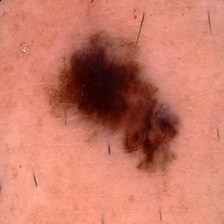
\includegraphics[width=4cm]{images/F01-A.png} 
	\end{center} 
	\vspace{-10pt}
	\caption{\footnotesize Melanoma maligno representado en el espacio RGB con una resolución de 224x244 píxeles almacenado en formato jpg.}  
	\label{fig01} 
\end{figure}

Podemos observar que en este primer método, los bordes se destacan de forma abrupta, obteniendo resultados poco suavizados y con una serie de disparos en el interior del área, los cuales nos gustaría evitar. Para mejorar esta propuesta, es posible segmentar el color de la imagen original mediante un algoritmo K-Means. Después de esta segmentación, se transforma la imagen a escala de grises. En esta etapa, reduciremos el rango dinámico para obtener una imagen binaria. Sin embargo, se observará que los resultados aún pueden mostrar cierta falta de suavidad en el contorno. Más adelante, se abordará una solución factible a este problema.

\begin{figure}[h] 
\begin{center} 
 \begin{tabular}{ccc}
        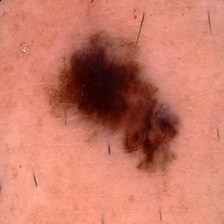
\includegraphics[width=2.4cm]{images/F01-A.png} &
        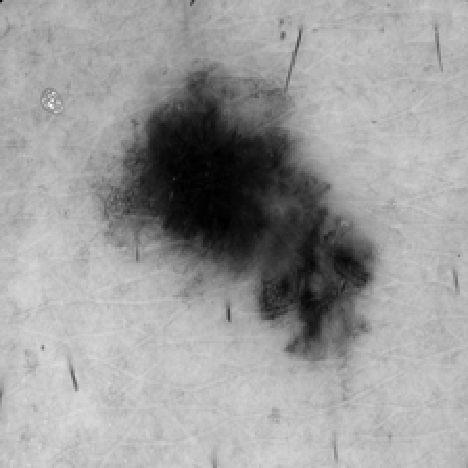
\includegraphics[width=2.4cm]{images/F01-B.png} & 
        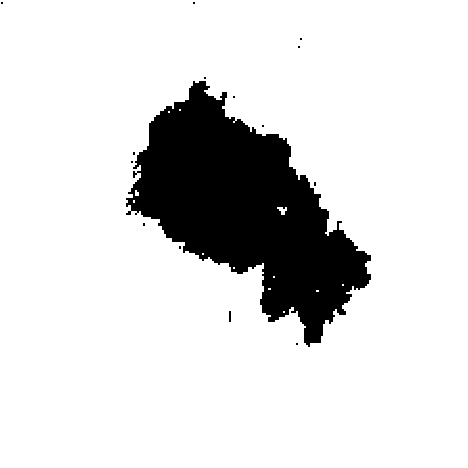
\includegraphics[width=2.4cm]{images/F01-C.png} \\
    (a) & (b) & (c)\\
  \end{tabular}
\end{center} 
\vspace{-10pt}
\caption{\footnotesize (a) Imagen original en el modelo RGB, (b) Imagen original en escala de grises, (c) Imagen en escala de grises con el rango dinámico reducido a dos valores (0 y 255).}  
\label{fig02} 
\end{figure}

\subsection{Implementación del Algoritmo K-Means}

La segmentación de color es una técnica utilizada en visión por computadora para identificar y distinguir diferentes objetos o regiones en una imagen basándose en sus colores \autocite{Anju:2019, Anju:2019, Dhanachandra:2015}. Los algoritmos de agrupamiento pueden separar automáticamente colores similares, sin necesidad de especificar valores de umbral para cada color. Esto puede ser útil al trabajar con imágenes que tienen una amplia gama de colores o cuando los valores de umbral exactos no se conocen de antemano \autocite{Bolat-2022}. 

El desarrollo completo de los algoritmos y métodos se llevará a cabo en MATLAB, por lo que se incorporarán fragmentos de código en este lenguaje. Inicialmente, definimos una función que requiere tres parámetros: la imagen original, el número deseado de grupos (indica la cantidad de tonalidades que tendrá la imagen resultante) y un número máximo de iteraciones para la segmentación. Dentro de la función se realizan las siguientes operaciones:

\begin{itemize}
    \item Se reorganiza la matriz originalImage en una nueva matriz con el número de filas igual al número total de elementos en originalImage y el número de columnas igual a 3 (una columna para cada canal de la imagen).
    \item De forma aleatoria, se seleccionan n índices de la matriz anterior, donde n corresponde al total de clústers. 
    \item En una nueva matriz ''centers'' de tres columnas se almacenan los valores de las $n$ posiciones aleatorias con los valores de los tres canales de color.
    \item Dentro de un ciclo for, en la variable ''D'' se calcula la distancia euclidiana entre los centros y cada píxel de la imagen, esto con ayuda de la función ''pdist2'' de MATLAB.
    \item Se actualizan los centros de los de los clústers. Para esto se crea un vector lógico donde todos los valores verdaderos son aquellos que pertenecen al cluster en ese punto de la iteración. Con esto, se pueden seleccionar todos los píxeles  de la imagen original que pertenecen a j. Por último se calcula la media de los píxeles seleccionados, esto actualiza el centro del cluster al promedio de las posiciones de los píxeles asignados a ese cluster.

    \begin{lstlisting}[style=Matlab-editor, caption=Fragmento del algoritmo K Means, basicstyle=\fontsize{8}{12}\selectfont]
    for iter=1:maxIter
        D = pdist2(centers,im2);
        [~,min_indices] = min(D);
        for j=1:clusterNo
            centers(j,:) = mean(im2(min_indices == j,:));
        end
    end
    \end{lstlisting}

    \item Se hace una asignación de colores a cada píxel según el cluster al que pertenece. Primero se  reorganiza la asignación de colores en la forma de la imagen original, se normalizan los valores de color a un rango de 0 a 1 y se acomodan en los tres canales de color.
\end{itemize}

De forma empírica se elige trabajar con 15 clústers y 100 iteraciones para el algoritmo. Las imágenes resultado donde este valor es ingresado de forma manual tendrán los valores mencionados. La imagen original en el modelo RGB (Figura~\ref{fig01}) segmentada con 15 clústers (Figura~\ref{fig03}) presenta ligeras variaciones en las tonalidades.

\begin{figure}[h] 
	\begin{center} 
		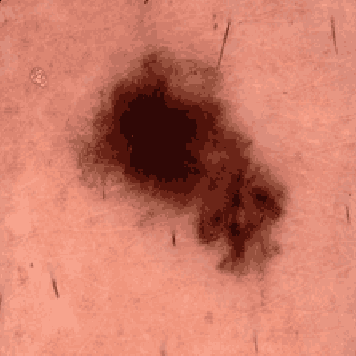
\includegraphics[width=4cm]{images/F03-A.png} 
	\end{center} 
	\vspace{-10pt}
	\caption{\footnotesize Imagen segmentada mediante el algoritmo K-Means con 15 clústers y 100 iteraciones.}  
	\label{fig03} 
\end{figure}

Si esta imagen la transformamos en una imagen en blanco y negro para después reducir su rango dinámico a dos, obtendríamos una imagen binaria con prevalecía de ruido en los alrededores y cambios abruptos en los bordes de la región principal (Figura~\ref{fig04}). Como solución a este problema se puede aplicar un filtro paso bajas butterworth a la imagen con el objetivo de suavizar y reducir elementos no deseados como lo son el ruido.  

\begin{figure}[h] 
\begin{center} 
 \begin{tabular}{cccc}
        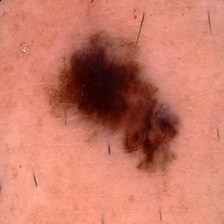
\includegraphics[width=1.7cm]{images/F01-A.png} &
        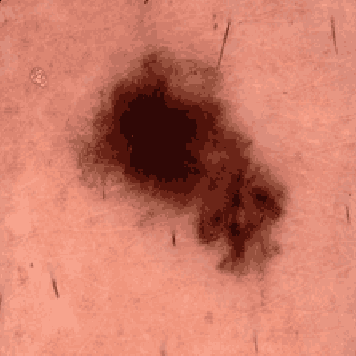
\includegraphics[width=1.7cm]{images/F03-A.png} & 
        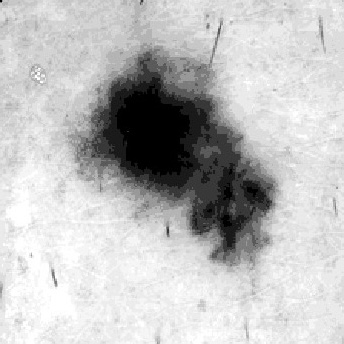
\includegraphics[width=1.7cm]{images/F04-A.png} & 
        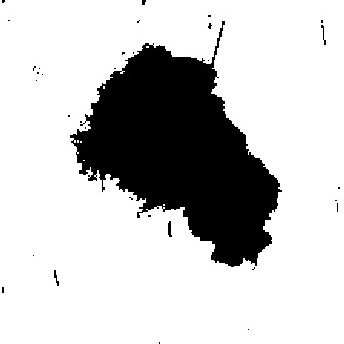
\includegraphics[width=1.7cm]{images/F04-B.png} \\
    (a) & (b) & (c) & (d)\\
  \end{tabular}
\end{center} 
\vspace{-10pt}
\caption{\footnotesize (a) Imagen original en el modelo RGB, (b) Imagen original segmentada en 15 clústers y 100 iteraciones, (c) Imagen segmentada en blanco y negro, (d) Imagen en blanco y negro con el rango dinámico reducido a dos valores.}  
\label{fig04} 
\end{figure}

\subsection{Implementación de un Filtro Paso Bajas Butterworth}

El filtro de paso bajas Butterworth se utiliza para suavizar la imagen en el dominio de la frecuencia. Elimina el ruido de alta frecuencia de una imagen digital y conserva los componentes de baja frecuencia \autocite{Makandar:2015, Gonzalez:2008}. Además sirve para suavizar la imagen mediante dos parámetros: frecuencia de corte y orden. En la evaluación de bordes, la implementación de este tipo de filtro será para suavizar el área alrededor del tumor para después obtener una imagen binaria a partir de este resultado, esperando obtener una silueta de color negro con el melanoma. 

\begin{figure}[h] 
\begin{tabular}{cc}
    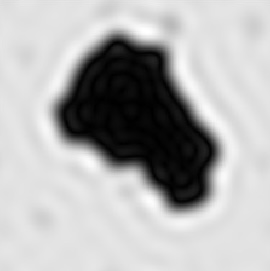
\includegraphics[width=1.7cm]{images/F05-A.png} &
    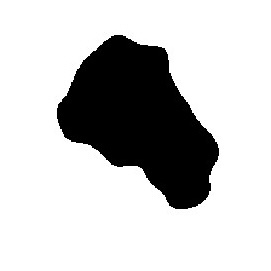
\includegraphics[width=1.7cm]{images/F05-B.jpeg} \\
    FC: 10 & Orden: 10 \\
    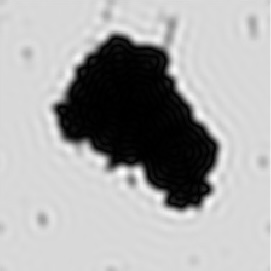
\includegraphics[width=1.7cm]{images/F05-C.png} & 
    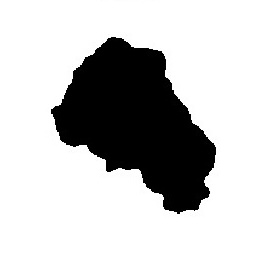
\includegraphics[width=1.7cm]{images/F05-D.jpeg} \\
    FC: 20 & Orden: 10 \\
    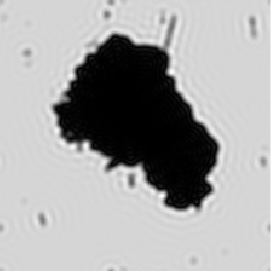
\includegraphics[width=1.7cm]{images/F05-E.png} &
    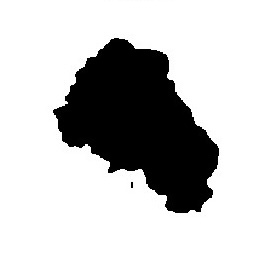
\includegraphics[width=1.7cm]{images/F05-F.jpeg} \\
    FC: 30 & Orden: 10 \\
    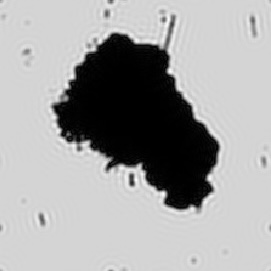
\includegraphics[width=1.7cm]{images/F05-G.jpeg} & 
    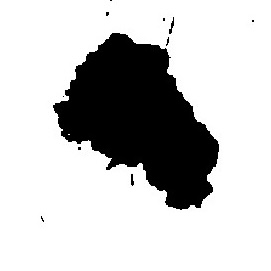
\includegraphics[width=1.7cm]{images/F05-H.jpeg} \\
    FC: 40 & Orden: 10 \\
\end{tabular}
\vspace{10pt}
\caption{\footnotesize A, C, E y G representan segmentaciones en blanco y negro, sometidas a un filtrado de paso bajo de orden 10 con frecuencias de corte de 10, 20, 30 y 40, respectivamente. B, D, F y H son imágenes binarias derivadas de las segmentaciones correspondientes A, C, E y G.}  
\label{fig05} 
\end{figure}

Para las imagenes anexadas en este reporte se decide usar una frecuencia de corte de 20 con orden igual a 10. Estos valores pueden ser manipulados con diferentes parámetros con el objetivo de obtener resultados más suavizados. En (Figura~\ref{fig05}) se puede ver el comportamiento cuando el valor de la frecuencia de corte se va modificando, en la primera columna se encuentra la imagen con el filtro paso bajas y en la segunda la misma imagen con un rango dinámico reducido.

 \begin{figure}[h] 
	\begin{center} 
		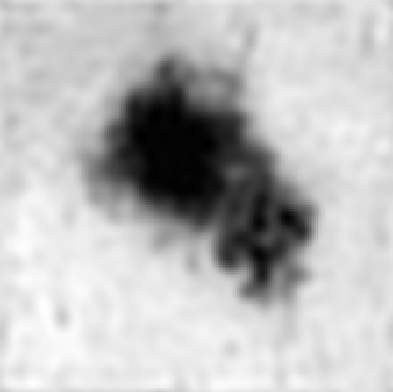
\includegraphics[width=4cm]{images/F06-A.png} 
	\end{center} 
	\vspace{-10pt}
	\caption{\footnotesize Melanoma maligno representado en escala de grises después de aplicar un filtro butterworth paso bajas de orden 10 con frecuencia de corte 20.}  
	\label{fig06} 
\end{figure}


En algunos casos el filtro es capaz de eliminar elementos no deseados que se encuentran situados en el exterior del área de interés. Esto aporta un gran valor sobre el resultado final pues es capaz de reducir filtraciones que dificulten diversos análisis como la evaluación de asimetría. Los resultados de este análisis abarcan desde la (Figura \ref{fig07}) hasta la (Figura \ref{fig11}).



\begin{figure*}
    \centering
    \begin{tabular}{cccccc}
        \adjustbox{valign=c}{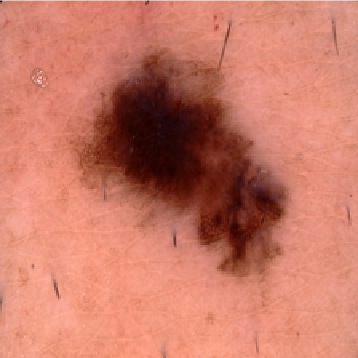
\includegraphics[width=1.7cm]{images/F07-A.png}} &
        \adjustbox{valign=c}{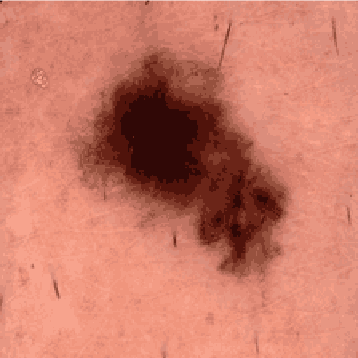
\includegraphics[width=1.7cm]{images/F07-B.png}} & 
        \adjustbox{valign=c}{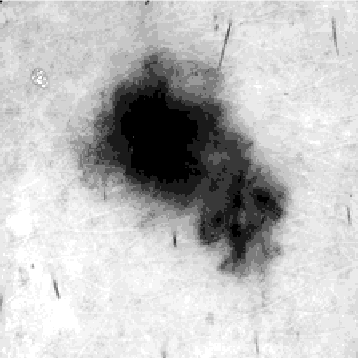
\includegraphics[width=1.7cm]{images/F07-C.png}} & 
        \adjustbox{valign=c}{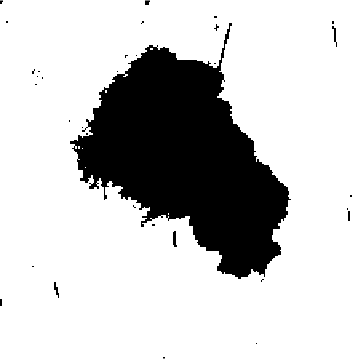
\includegraphics[width=1.7cm]{images/F07-D.png}} &
        \adjustbox{valign=c}{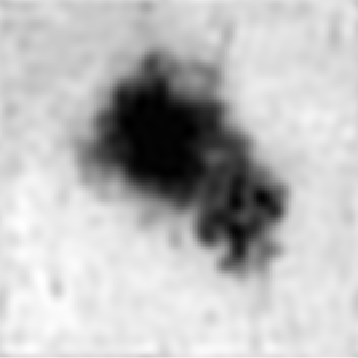
\includegraphics[width=1.7cm]{images/F07-E.png}} & 
        \adjustbox{valign=c}{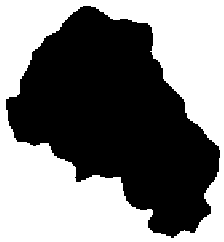
\includegraphics[width=1.3cm]{images/F07-F.png}} \\
        (a) & (b) & (c) & (d) & (e) & (f)\\
    \end{tabular}
    \caption{\footnotesize (a) imagen en el modelo RGB, (b) segmentación de color con K Medias, (c) imagen segmentada en blanco y negro, (d) imagen en blanco y negro con valores ecualizados, (e) imagen con valores ecualizados con trasnformación binaria, (f) imagen con filtro paso bajas.}  
    \label{fig07} 
\end{figure*}

\begin{figure*}
    \centering
    \begin{tabular}{cccccc}
        \adjustbox{valign=c}{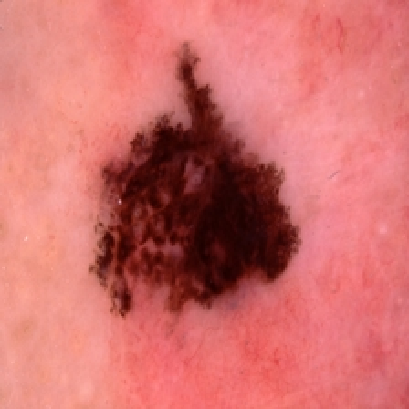
\includegraphics[width=1.7cm]{images/F08-A.png}} &
        \adjustbox{valign=c}{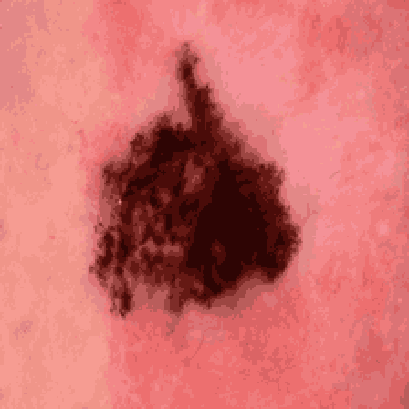
\includegraphics[width=1.7cm]{images/F08-B.png}} & 
        \adjustbox{valign=c}{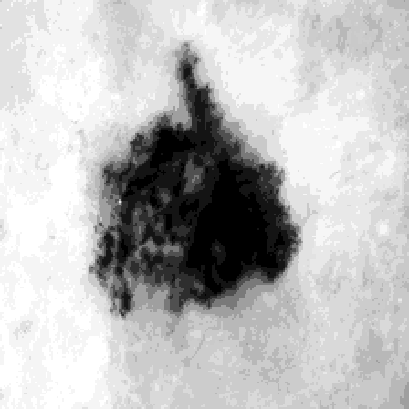
\includegraphics[width=1.7cm]{images/F08-C.png}} & 
        \adjustbox{valign=c}{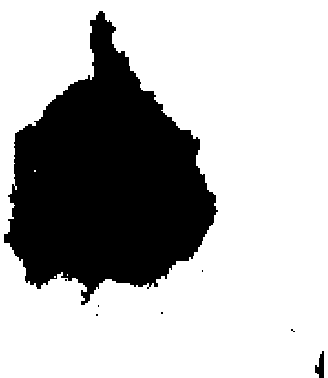
\includegraphics[width=1.5cm]{images/F08-D.png}} &
        \adjustbox{valign=c}{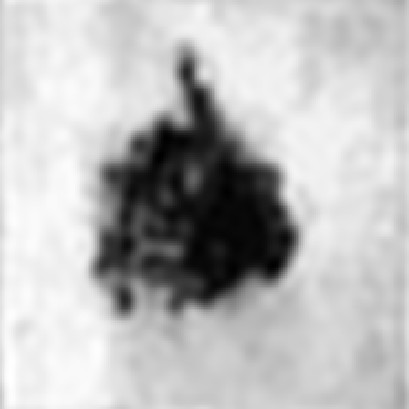
\includegraphics[width=1.7cm]{images/F08-E.png}} & 
        \adjustbox{valign=c}{
\includegraphics[width=1.3cm]{images/F08-F.png}} \\
        (a) & (b) & (c) & (d) & (e) & (f)\\
    \end{tabular}
    \caption{\footnotesize (a) imagen en el modelo HSI, (b) segmentación de color con K Medias, (c) imagen segmentada en blanco y negro, (d) imagen en blanco y negro con valores ecualizados, (e) imagen con valores ecualizados con trasnformación binaria, (f) imagen con filtro paso bajas.}  
    \label{fig08} 
\end{figure*}

\begin{figure*}
    \centering
    \begin{tabular}{cccccc}
        \adjustbox{valign=c}{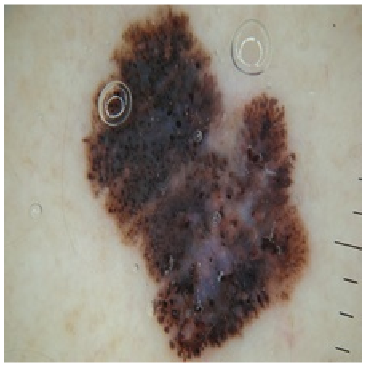
\includegraphics[width=1.7cm]{images/F09-A.png}} &
        \adjustbox{valign=c}{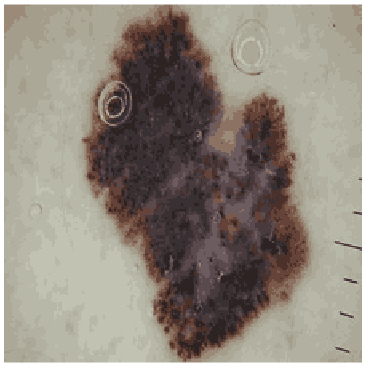
\includegraphics[width=1.7cm]{images/F09-B.png}} & 
        \adjustbox{valign=c}{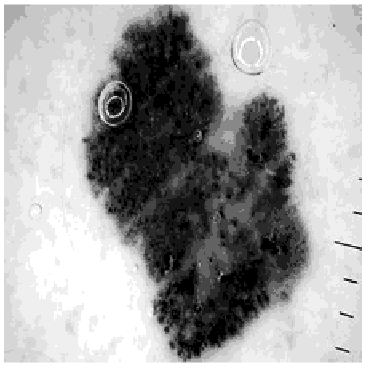
\includegraphics[width=1.7cm]{images/F09-C.png}} & 
        \adjustbox{valign=c}{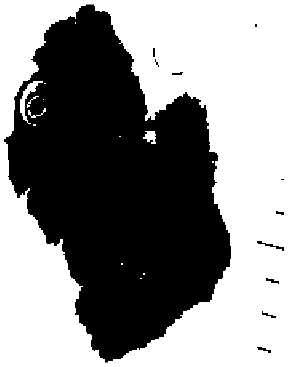
\includegraphics[width=1.2cm]{images/F09-D.png}} &
        \adjustbox{valign=c}{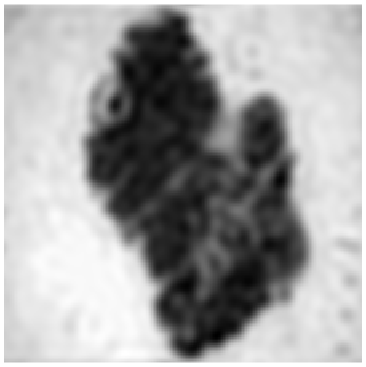
\includegraphics[width=1.7cm]{images/F09-E.png}} & 
        \adjustbox{valign=c}{
\includegraphics[width=0.9cm]{images/F09-F.png}} \\
        (a) & (b) & (c) & (d) & (e) & (f)\\
    \end{tabular}
    \caption{\footnotesize (a) imagen en el modelo HSI, (b) segmentación de color con K Medias, (c) imagen segmentada en blanco y negro, (d) imagen en blanco y negro con valores ecualizados, (e) imagen con valores ecualizados con trasnformación binaria, (f) imagen con filtro paso bajas.}  
    \label{fig09} 
\end{figure*}

\begin{figure*}
    \centering
    \begin{tabular}{cccccc}
        \adjustbox{valign=c}{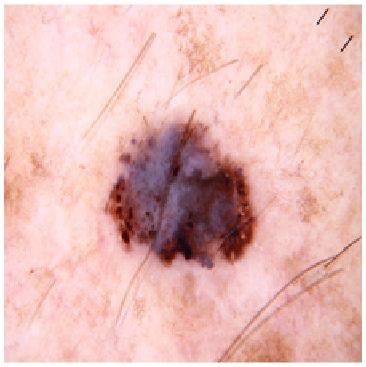
\includegraphics[width=1.7cm]{images/F10-A.png}} &
        \adjustbox{valign=c}{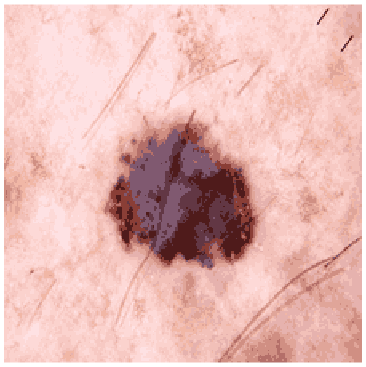
\includegraphics[width=1.7cm]{images/F10-B.png}} & 
        \adjustbox{valign=c}{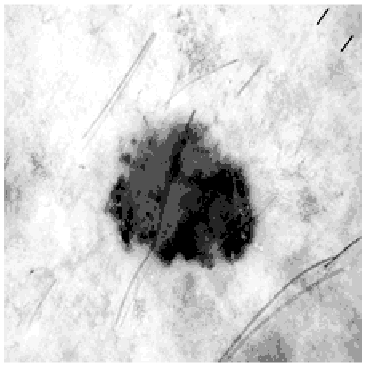
\includegraphics[width=1.7cm]{images/F10-C.png}} & 
        \adjustbox{valign=c}{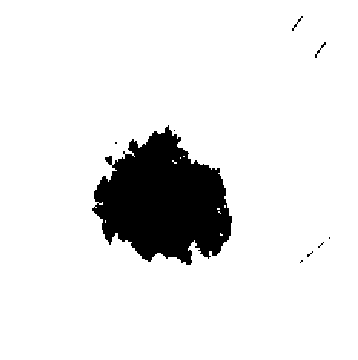
\includegraphics[width=1.7cm]{images/F10-D.png}} &
        \adjustbox{valign=c}{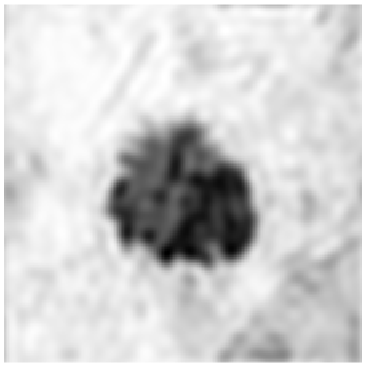
\includegraphics[width=1.7cm]{images/F10-E.png}} & 
        \adjustbox{valign=c}{
\includegraphics[width=0.8cm]{images/F10-F.png}} \\
        (a) & (b) & (c) & (d) & (e) & (f)\\
    \end{tabular}
    \caption{\footnotesize (a) imagen en el modelo HSI, (b) segmentación de color con K Medias, (c) imagen segmentada en blanco y negro, (d) imagen en blanco y negro con valores ecualizados, (e) imagen con valores ecualizados con trasnformación binaria, (f) imagen con filtro paso bajas.}  
    \label{fig10} 
\end{figure*}

\begin{figure*}
    \centering
    \begin{tabular}{cccccc}
        \adjustbox{valign=c}{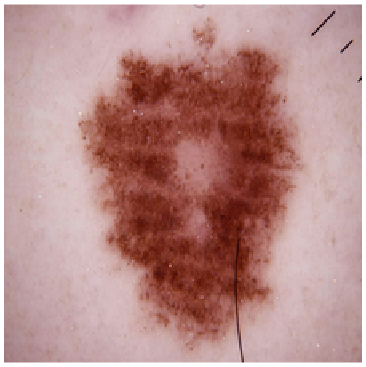
\includegraphics[width=1.7cm]{images/F11-A.png}} &
        \adjustbox{valign=c}{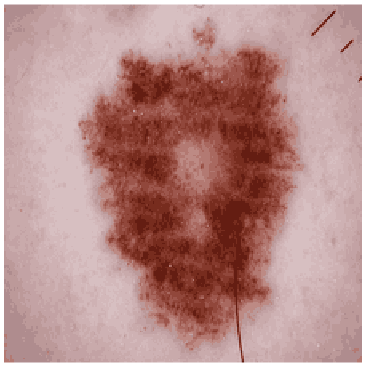
\includegraphics[width=1.7cm]{images/F11-B.png}} & 
        \adjustbox{valign=c}{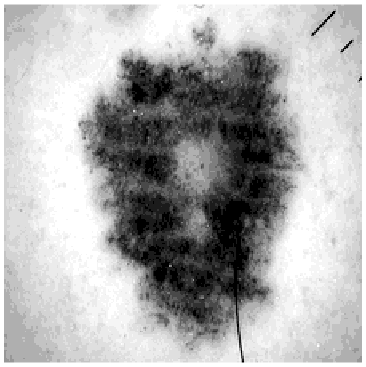
\includegraphics[width=1.7cm]{images/F11-C.png}} & 
        \adjustbox{valign=c}{
\includegraphics[width=1.5cm]{images/F11-D.png}} &
        \adjustbox{valign=c}{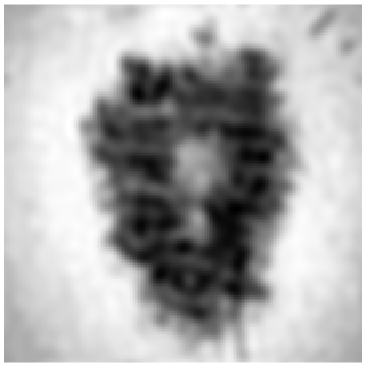
\includegraphics[width=1.7cm]{images/F11-E.png}} & 
        \adjustbox{valign=c}{
\includegraphics[width=1cm]{images/F11-F.png}} \\
        (a) & (b) & (c) & (d) & (e) & (f)\\
    \end{tabular}
    \caption{\footnotesize (a) imagen en el modelo HSI, (b) segmentación de color con K Medias, (c) imagen segmentada en blanco y negro, (d) imagen en blanco y negro con valores ecualizados, (e) imagen con valores ecualizados con trasnformación binaria, (f) imagen con filtro paso bajas.}  
    \label{fig11} 
\end{figure*}

\clearpage

\subsection{Evaluación de desempeño en el modelo HSI}

En el modelo HSI, los colores se definen mediante su tono, saturación e intensidad, aspectos intrínsecamente vinculados a la percepción humana del color \autocite{Rojas:2008}. El propósito de esta sección radica en evaluar de manera subjetiva los efectos resultantes de las manipulaciones de la imagen en comparación con el modelo RGB. Para ello, es necesario obtener una imagen que siga el esquema del modelo HSI. Se hace uso de una función de implementación propia que toma como parámetro una imagen en formato RGB y devuelve la misma imagen en el modelo HSI. En esta función, se lleva a cabo la normalización de los valores de RGB, ajustándolos al rango de 0 a 1. Posteriormente, se procede a descomponer la imagen en sus tres canales de color: R (rojo), G (verde) y B (azul). Se calcula el ángulo theta, que representa la matiz H, mediante una fórmula que incluye las diferencias entre los canales de color.

Se realiza una corrección en el valor de H para asegurar que se encuentre en el rango de 0 a 2 por el valor de pi. La saturación S se determina como 1 menos el valor mínimo entre los tres canales, dividido por la suma de los tres canales. Finalmente, la intensidad I se obtiene como el promedio de los valores de los canales R, G y B. En la última etapa, se utiliza la función ''cat'' para combinar los resultados de H, S e I en una nueva imagen en formato HSI.

 \begin{lstlisting}[style=Matlab-editor, caption=Fragmento del algoritmo K Means, basicstyle=\fontsize{8}{12}\selectfont]
function hsi = rgbTohsi(rgb)
    rgb = double(rgb) / 255;
    r = rgb(:,:,1);
    g = rgb(:,:,2);
    b = rgb(:,:,3);

    num = 0.5 * ((r - g) + (r - b));
    den = sqrt((r - g).^2 + (r - b).*(g - b));
    theta = acos(num ./ (den + eps));

    h = theta;
    h(b > g) = 2*pi - h(b > g); 
    h = h / (2*pi);
 
    s = 1 - 3 * min(rgb, [], 3) ./ sum(rgb, 3);
    i = (r + g + b) / 3;
    hsi = cat(3, h, s, i);
end
\end{lstlisting}

La (Figura~\ref{fig12}) muestra la representación visual del objeto de estudio, conforme al nuevo modelo de color que se ha empleado a lo largo del presente escrito. En (Figura~\ref{fig13}) a (Figura~\ref{fig17}) se detallan los resultados derivados de la aplicación de los procedimientos aludidos en este nuevo espacio cromático. A pesar de la congruencia observada en ciertas instancias, en otras, la semejanza tonal compromete la eficacia de los algoritmos para alcanzar los propósitos iniciales delineados.


\begin{figure}
		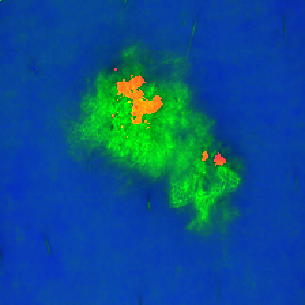
\includegraphics[width=4cm]{images/F12.png} 
\caption{Melanoma maligno representado en el espacio HSI con una resolución de 224 x 244 píxeles almacenado en formato jpg.}
\label{fig12}
\end{figure}

 
% FIGURA 13
\begin{figure*}
    \centering
    \begin{tabular}{cccccccc}
        \adjustbox{valign=c}{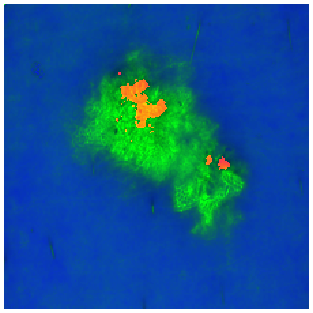
\includegraphics[width=1.5cm]{images/F13-A.png}} &
        \adjustbox{valign=c}{\includegraphics[width=1.5cm]{images/F13-B.png}} & 
        \adjustbox{valign=c}{\includegraphics[width=1.5cm]{images/F13-C.png}} & 
        \adjustbox{valign=c}{\includegraphics[width=1.5cm]{images/F13-D.png}} &
        \adjustbox{valign=c}{\includegraphics[width=1.5cm]{images/F13-E.png}} & 
        \adjustbox{valign=c}{\includegraphics[width=1.5cm]{images/F13-E.png}} & 
		\adjustbox{valign=c}{\includegraphics[width=1.5cm]{images/F13-F.png}} & 
        \adjustbox{valign=c}{\includegraphics[width=1.5cm]{images/F13-G.png}} \\
        (a) & (b) & (c) & (d) & (e) & (f) & (g) & (h)\\
    \end{tabular}
    \caption{\footnotesize A: imagen en el modelo HSI, B: segmentación de color con K Menas, C: imagen segmentada en blanco y negro, D: imagen en blanco y negro con valores ecualizados, E: imagen binaria de D, E: imagen con filtro paso bajas de C, F: imagen binaria de E, G: imagen con filtro butterworth de orden 10 y frecuencia de corte 20,H: imagen binaria de G}  
    \label{fig13} 
\end{figure*}

% FIGURA 14
\begin{figure*}
    \centering
    \begin{tabular}{cccccccc}
        \adjustbox{valign=c}{\includegraphics[width=1.5cm]{images/F14-A.png}} &
        \adjustbox{valign=c}{\includegraphics[width=1.5cm]{images/F14-B.png}} & 
        \adjustbox{valign=c}{\includegraphics[width=1.5cm]{images/F14-C.png}} & 
        \adjustbox{valign=c}{\includegraphics[width=1.5cm]{images/F14-D.png}} &
        \adjustbox{valign=c}{\includegraphics[width=1.5cm]{images/F14-E.png}} & 
        \adjustbox{valign=c}{\includegraphics[width=1.5cm]{images/F14-E.png}} & 
		\adjustbox{valign=c}{\includegraphics[width=1.5cm]{images/F14-F.png}} & 
        \adjustbox{valign=c}{\includegraphics[width=1.5cm]{images/F14-G.png}} \\
        (a) & (b) & (c) & (d) & (e) & (f) & (g) & (h)\\
    \end{tabular}
    \caption{\footnotesize (a) imagen en el modelo HSI, (b) segmentación de color con K Menas, (c) imagen segmentada en blanco y negro, (d) imagen en blanco y negro con valores ecualizados, E: imagen binaria de d, (e) imagen con filtro paso bajas de c, (f) imagen binaria de e, (g) imagen con filtro butterworth de orden 10 y frecuencia de corte 20, (h) imagen binaria de g.}  
    \label{fig14} 
\end{figure*}



% FIGURA 15
\begin{figure*}
    \centering
    \begin{tabular}{cccccccc}
        \adjustbox{valign=c}{\includegraphics[width=1.5cm]{images/F15-A.png}} &
        \adjustbox{valign=c}{\includegraphics[width=1.5cm]{images/F15-B.png}} & 
        \adjustbox{valign=c}{\includegraphics[width=1.5cm]{images/F15-C.png}} & 
        \adjustbox{valign=c}{\includegraphics[width=1.5cm]{images/F15-D.png}} &
        \adjustbox{valign=c}{\includegraphics[width=1.5cm]{images/F15-E.png}} & 
        \adjustbox{valign=c}{\includegraphics[width=1.5cm]{images/F15-E.png}} & 
		\adjustbox{valign=c}{\includegraphics[width=1.5cm]{images/F15-F.png}} & 
        \adjustbox{valign=c}{\includegraphics[width=1.5cm]{images/F15-G.png}} \\
        (a) & (b) & (c) & (d) & (e) & (f) & (g) & (h)\\
    \end{tabular}
    \caption{\footnotesize (a) imagen en el modelo HSI, (b) segmentación de color con K Menas, (c) imagen segmentada en blanco y negro, (d) imagen en blanco y negro con valores ecualizados, E: imagen binaria de d, (e) imagen con filtro paso bajas de c, (f) imagen binaria de e, (g) imagen con filtro butterworth de orden 10 y frecuencia de corte 20, (h) imagen binaria de g.}  
    \label{fig15} 
\end{figure*}

% FIGURA 16
\begin{figure*}
    \centering
    \begin{tabular}{cccccccc}
        \adjustbox{valign=c}{\includegraphics[width=1.5cm]{images/F16-A.png}} &
        \adjustbox{valign=c}{\includegraphics[width=1.5cm]{images/F16-B.png}} & 
        \adjustbox{valign=c}{\includegraphics[width=1.5cm]{images/F16-C.png}} & 
        \adjustbox{valign=c}{\includegraphics[width=1.5cm]{images/F16-D.png}} &
        \adjustbox{valign=c}{\includegraphics[width=1.5cm]{images/F16-E.png}} & 
        \adjustbox{valign=c}{\includegraphics[width=1.5cm]{images/F16-E.png}} & 
		\adjustbox{valign=c}{\includegraphics[width=1.5cm]{images/F16-F.png}} & 
        \adjustbox{valign=c}{\includegraphics[width=1.5cm]{images/F16-G.png}} \\
        (a) & (b) & (c) & (d) & (e) & (f) & (g) & (h)\\
    \end{tabular}
    \caption{\footnotesize (a) imagen en el modelo HSI, (b) segmentación de color con K Menas, (c) imagen segmentada en blanco y negro, (d) imagen en blanco y negro con valores ecualizados, E: imagen binaria de d, (e) imagen con filtro paso bajas de c, (f) imagen binaria de e, (g) imagen con filtro butterworth de orden 10 y frecuencia de corte 20, (h) imagen binaria de g.}   
    \label{fig16} 
\end{figure*}

% FIGURA 17
\begin{figure*}
    \centering
    \begin{tabular}{cccccccc}
        \adjustbox{valign=c}{\includegraphics[width=1.5cm]{images/F17-A.png}} &
        \adjustbox{valign=c}{\includegraphics[width=1.5cm]{images/F17-B.png}} & 
        \adjustbox{valign=c}{\includegraphics[width=1.5cm]{images/F17-C.png}} & 
        \adjustbox{valign=c}{\includegraphics[width=1.5cm]{images/F17-D.png}} &
        \adjustbox{valign=c}{\includegraphics[width=1.5cm]{images/F17-E.png}} & 
        \adjustbox{valign=c}{\includegraphics[width=1.5cm]{images/F17-E.png}} & 
		\adjustbox{valign=c}{\includegraphics[width=1.5cm]{images/F17-F.png}} & 
        \adjustbox{valign=c}{\includegraphics[width=1.5cm]{images/F17-G.png}} \\
        (a) & (b) & (c) & (d) & (e) & (f) & (g) & (h)\\
    \end{tabular}
    \caption{\footnotesize (a) imagen en el modelo HSI, (b) segmentación de color con K Menas, (c) imagen segmentada en blanco y negro, (d) imagen en blanco y negro con valores ecualizados, E: imagen binaria de d, (e) imagen con filtro paso bajas de c, (f) imagen binaria de e, (g) imagen con filtro butterworth de orden 10 y frecuencia de corte 20, (h) imagen binaria de g.}  
    \label{fig17} 
\end{figure*}


\clearpage
\section{Análisis de Color}

Para analizar este atributo, emplearemos el algoritmo de segmentación. No obstante, con el fin de mejorar su rendimiento, se implementará una versión que no requiera la introducción manual del número de clústers. Hasta este punto, todas las imágenes se han segmentado utilizando 15 clústeres; no obstante, más adelante llevaremos a cabo una comparativa entre el valor original y el número óptimo obtenido con este nuevo método.


\subsection{Selección óptima de clústeres con el método del Codo}

El método del codo es una técnica gráfica utilizada para determinar el número óptimo de clústeres (K) en el algoritmo de agrupamiento K-means. Este método se basa en la búsqueda de la suma de los cuadrados intra-cluster (WCSS, por sus siglas en inglés), que representa la suma de las distancias al cuadrado entre los puntos de un clúster y el centroide de ese clúster \autocite{Zheng:2018}.

En el proceso de K-means, se prueban diferentes valores de K para dividir el conjunto de datos en un número específico de clústeres. Para cada valor de K, se calcula el WCSS. El WCSS disminuirá a medida que aumente K, ya que cada punto estará más cerca de su centroide en clústeres más pequeños \autocite{Anju:2019}. Sin embargo, llegará un punto en el que el incremento adicional en K no conllevará una reducción significativa en el WCSS \autocite{Dhanachandra:2015}.

La representación gráfica de esta relación entre el número de clústeres y el WCSS se asemeja a la forma de un ''codo'' en una gráfica, como se puede observar en la figura dieciocho. El punto en el que se observa una desaceleración en la disminución del WCSS y la curva parece formar un codo es considerado como el número óptimo de clústeres para el conjunto de \autocite{Sammouda:2021}. Para la implementación de este algoritmo se define una función que recibe tres parámetros:

\begin{itemize}
    \item originalImage: imagen original que se utilizará para el análisis.
    \item maxClusters: número máximo de clústers que se probarán. En este caso, todas las imágenes tendrán con máximo 15 unidades, para una mejor comparativa con los resultados originales.
    \item maxIter: número máximo de iteraciones para el algoritmo de k-means en cada prueba de clúster.
\end{itemize}

\noindent Dentro de la función se realizan las siguientes operaciones:

\begin{itemize}
    \item Convertimos la imagen original en una matriz de dos dimensiones y se normaliza dividiendo cada valor por 255.
    \item Obtener el número de píxeles con la función numel
    \item Mediante un ciclo for sobre el rango de clústers desde 1 hasta maxClusters. Para cada número de clústers, se inicializan centroides de clústeres de manera aleatoria con ayuda de randperm.
    \item Se ejecuta el algoritmo de k-means en maxIter iteraciones.
    \item La distorsión, que es la suma de los cuadrados de las distancias mínimas al cuadrado se calcula y almacena para evaluar la ''calidad'' del agrupamiento.

     \begin{lstlisting}[style=Matlab-editor, caption=Fragmento del algoritmo findOptimalCluster, basicstyle=\fontsize{8}{12}\selectfont]
for k = 1:maxClusters
    randIndices = randperm(pixelNo, k);
    centers = im2(randIndices);

    for iter = 1:maxIter
        D = pdist2(centers, im2);
       [~, min_indices] = min(D);

        for j = 1:k
            centers(j) = mean(im2(min_indices == j));
        end
    end

    distortions(k) = sum(min(D).^2) / pixelNo;
end
\end{lstlisting}

    \item Se gráfican los resultados obtenidos de la distorsión, se encuentra el codo de los resultados con la primera derivada. Para esto se usa una función adicional 'findKnee'

\begin{lstlisting}[style=Matlab-editor, caption=Algoritmo findKnee, basicstyle=\fontsize{8}{12}\selectfont]
function [x, y] = findKnee(xValues)
    dx = xValues(2:end) - xValues(1:end-1);
    dy = diff(dx);
    [~, idx] = max(dy); 
    x = idx + 1;  
    y = xValues(x);
end
\end{lstlisting}

\end{itemize}


\begin{figure}
		\includegraphics[width=8cm]{images/F18.jpg} 
\caption{Gráfica para evaluar el número óptimo de clústers. Sobre el eje horizontal se encuentra el número de clústers, el eje vertical muestra la desviación sobre el valor K. En este caso el bajo el método del codo el número óptimo es cinco.}
\label{fig18}
\end{figure}

En (Figura~\ref{fig19}) se presenta una comparativa con la selección óptima de clústeres, donde se destaca el rendimiento satisfactorio cuando hay un número elevado de clústeres y cuando se segmenta con el valor óptimo. No obstante, se muestra que al incrementar este valor tareas como la segmentación por color o la compresión de imágenes se ven afectadas. No solo eso, mediante el método del codo se logran conservar los atributos necesarios para resaltar los bordes con una reducción considerable de información. Los resultados de este análisis abarcan desde la (Figura \ref{fig22}) hasta la (Figura \ref{fig26}).


% Figura 19
\begin{figure}[h] 
\begin{tabular}{cc}
    \textbf{15 clústers} & \textbf{Óptimo: 5} \\
    \includegraphics[width=1.7cm]{images/F19-A.jpg} &
    \includegraphics[width=1.7cm]{images/F19-B.jpg} \\
    \textbf{15 clústers} & \textbf{Óptimo: 5} \\
    \includegraphics[width=1.7cm]{images/F19-C.jpg} & 
    \includegraphics[width=1.7cm]{images/F19-D.jpg} \\
	\textbf{15 clústers} & \textbf{Óptimo: 3} \\
    \includegraphics[width=1.7cm]{images/F19-E.jpg} &
    \includegraphics[width=1.7cm]{images/F19-F.jpg} \\
	\textbf{15 clústers} & \textbf{Óptimo: 6} \\
    \includegraphics[width=1.7cm]{images/F19-G.jpg} & 
    \includegraphics[width=1.7cm]{images/F19-H.jpg} \\
	\textbf{15 clústers} & \textbf{Óptimo: 5} \\
	\includegraphics[width=1.7cm]{images/F19-I.jpg} & 
    \includegraphics[width=1.7cm]{images/F19-J.jpg} \\
\end{tabular}
\caption{Comparación de uso con selección óptima de clústeres: las imá- genes en la columna izquierda fueron segmentadas con 15 clústers, mientras que las de la derecha utilizaron un valor obtenido mediante el método del codo, indicando en su etiqueta el número de clústers}  
\label{fig19} 
\end{figure}

La figura diseñada para el análisis de color, presenta cada uno de los colores segregados de la imagen original en una única fila utilizando el método para obtener el método óptimo de clústers. Para un análisis más enriquecedor, se decide mostrar los colores segmentados con dos fondos distintos: blanco y negro. Ambos resultados pueden verse en   (Figura~\ref{fig20}) y (Figura~\ref{fig21}). 

% Figura 20
\begin{figure}
    \centering
    \begin{tabular}{ccccc}
        \adjustbox{valign=c}{\includegraphics[width=1.3cm]{images/F20-A.png}} &
        \adjustbox{valign=c}{\includegraphics[width=1.3cm]{images/F20-B.png}} & 
        \adjustbox{valign=c}{\includegraphics[width=1.3cm]{images/F20-C.png}} & 
		\adjustbox{valign=c}{\includegraphics[width=1.3cm]{images/F20-D.png}} & 
        \adjustbox{valign=c}{\includegraphics[width=1.3cm]{images/F20-E.png}} \\
        (a) & (b) & (c) & (d) & (e)\\
    \end{tabular}
    \caption{\footnotesize Colores segmentados de la imagen original con el método del codo, el área que no corresponde al color segmentado se aprecia de color negro.}  
    \label{fig20} 
\end{figure}

% Figura 21
\begin{figure}
    \centering
    \begin{tabular}{ccccc}
        \adjustbox{valign=c}{\includegraphics[width=1.3cm]{images/F21-A.png}} &
        \adjustbox{valign=c}{\includegraphics[width=1.3cm]{images/F21-B.png}} & 
        \adjustbox{valign=c}{\includegraphics[width=1.3cm]{images/F21-C.png}} & 
		\adjustbox{valign=c}{\includegraphics[width=1.3cm]{images/F21-D.png}} & 
        \adjustbox{valign=c}{\includegraphics[width=1.3cm]{images/F21-E.png}} \\
        (a) & (b) & (c) & (d) & (e) \\
    \end{tabular}
    \caption{\footnotesize Colores segmentados de la imagen original con el método del codo, el área que no corresponde al color segmentado se aprecia de color blanco.}  
    \label{fig21} 
\end{figure}


% FIGURA 22
\begin{figure*}
    \centering
    \begin{tabular}{cccccc}
        \adjustbox{valign=c}{\includegraphics[width=2cm]{images/F22-A.png}} & 
        \adjustbox{valign=c}{\includegraphics[width=2cm]{images/F22-B.png}} &
        \adjustbox{valign=c}{\includegraphics[width=2cm]{images/F22-C.png}} & 
        \adjustbox{valign=c}{\includegraphics[width=1.5cm]{images/F22-D.png}} & 
		\adjustbox{valign=c}{\includegraphics[width=2cm]{images/F22-E.png}} & 
        \adjustbox{valign=c}{\includegraphics[width=1.2cm]{images/F22-F.png}} \\
        (a) & (b) & (c) & (d) & (e) & (f)\\
    \end{tabular}
    \caption{\footnotesize A: imagen en el modelo HSI, B: segmentación de color con K Menas, C: imagen B en blanco y negro, D: imagen C con valores ecualizados, E: imagen binaria de D, E: imagen paso bajas de C, F: imagen binaria de E}
    \label{fig22} 
\end{figure*}

% FIGURA 23
\begin{figure*}
    \centering
    \begin{tabular}{cccccc}
        \adjustbox{valign=c}{\includegraphics[width=2cm]{images/F23-A.png}} & 
        \adjustbox{valign=c}{\includegraphics[width=2cm]{images/F23-B.png}} &
        \adjustbox{valign=c}{\includegraphics[width=2cm]{images/F23-C.png}} & 
        \adjustbox{valign=c}{\includegraphics[width=1.5cm]{images/F23-D.png}} & 
		\adjustbox{valign=c}{\includegraphics[width=2cm]{images/F23-E.png}} & 
        \adjustbox{valign=c}{\includegraphics[width=1.5cm]{images/F23-F.png}} \\
        (a) & (b) & (c) & (d) & (e) & (f)\\
    \end{tabular}
    \caption{\footnotesize A: imagen en el modelo HSI, B: segmentación de color con K Menas, C: imagen B en blanco y negro, D: imagen C con valores ecualizados, E: imagen binaria de D, E: imagen paso bajas de C, F: imagen binaria de E}
    \label{fig23} 
\end{figure*}

% FIGURA 24
\begin{figure*}
    \centering
    \begin{tabular}{cccccc}
        \adjustbox{valign=c}{\includegraphics[width=2cm]{images/F24-A.png}} & 
        \adjustbox{valign=c}{\includegraphics[width=2cm]{images/F24-B.png}} &
        \adjustbox{valign=c}{\includegraphics[width=2cm]{images/F24-C.png}} & 
        \adjustbox{valign=c}{\includegraphics[width=1.5cm]{images/F24-D.png}} & 
		\adjustbox{valign=c}{\includegraphics[width=2cm]{images/F24-E.png}} & 
        \adjustbox{valign=c}{\includegraphics[width=1cm]{images/F24-F.png}} \\
        (a) & (b) & (c) & (d) & (e) & (f)\\
    \end{tabular}
    \caption{\footnotesize A: imagen en el modelo HSI, B: segmentación de color con K Menas, C: imagen B en blanco y negro, D: imagen C con valores ecualizados, E: imagen binaria de D, E: imagen paso bajas de C, F: imagen binaria de E}
    \label{fig24} 
\end{figure*}

% FIGURA 25
\begin{figure*}
    \centering
    \begin{tabular}{cccccc}
        \adjustbox{valign=c}{\includegraphics[width=2cm]{images/F25-A.png}} & 
        \adjustbox{valign=c}{\includegraphics[width=2cm]{images/F25-B.png}} &
        \adjustbox{valign=c}{\includegraphics[width=2cm]{images/F25-C.png}} & 
        \adjustbox{valign=c}{\includegraphics[width=1.5cm]{images/F25-D.png}} & 
		\adjustbox{valign=c}{\includegraphics[width=2cm]{images/F25-E.png}} & 
        \adjustbox{valign=c}{\includegraphics[width=1cm]{images/F25-F.png}} \\
        (a) & (b) & (c) & (d) & (e) & (f)\\
    \end{tabular}
    \caption{\footnotesize A: imagen en el modelo HSI, B: segmentación de color con K Menas, C: imagen B en blanco y negro, D: imagen C con valores ecualizados, E: imagen binaria de D, E: imagen paso bajas de C, F: imagen binaria de E}
    \label{fig25} 
\end{figure*}

% FIGURA 26
\begin{figure*}
    \centering
    \begin{tabular}{cccccc}
        \adjustbox{valign=c}{\includegraphics[width=2cm]{images/F26-A.png}} & 
        \adjustbox{valign=c}{\includegraphics[width=2cm]{images/F26-B.png}} &
        \adjustbox{valign=c}{\includegraphics[width=2cm]{images/F26-C.png}} & 
        \adjustbox{valign=c}{\includegraphics[width=1.5cm]{images/F26-D.png}} & 
		\adjustbox{valign=c}{\includegraphics[width=2cm]{images/F26-E.png}} & 
        \adjustbox{valign=c}{\includegraphics[width=1cm]{images/F26-F.png}} \\
        (a) & (b) & (c) & (d) & (e) & (f)\\
    \end{tabular}
    \caption{\footnotesize A: imagen en el modelo HSI, B: segmentación de color con K Menas, C: imagen B en blanco y negro, D: imagen C con valores ecualizados, E: imagen binaria de D, E: imagen paso bajas de C, F: imagen binaria de E}
    \label{fig26} 
\end{figure*}




\clearpage


\section{Conclusiones}

Se comprobó de manera empírica que las variaciones en los resultados pueden depender del modelo de color presente en la imagen a manipular. En situaciones donde las imágenes muestran colores muy similares o ligeras variaciones en sus tonalidades en la región de interés, el modelo HSI resulta menos útil al absorber parte de estos cambios cromáticos. No obstante, se observa una notable mejora en el rendimiento del algoritmo de segmentación en comparación con los resultados obtenidos mediante el modelo RGB. Es posible que el desempeño varíe según el área de aplicación y el modelo utilizado, razón por la cual se recomienda un análisis detallado de su comportamiento antes de llegar a una conclusión sobre un solo modelo.

El desarrollo de la práctica transcurrió sin contratiempos y fue posible consolidar de manera efectiva todos los conocimientos adquiridos a lo largo del curso. 
\section{Código}
Todo los scripts y funciones implementadas para el desarrollo de la práctica pueden ser consultados en el siguiente repositorio remoto. \href{https://github.com/Ramon-OC/Melanoma-Analysis}{\textbf{Haga click aquí: } \textcolor{blue}{Melanoma-Analysis GitHub}}. 

\printendnotes

\printbibliography

\end{document}